\section{Introduction}
\label{sec:intro}
Butterfly computation is a common building block in scientific computing,
machine learning, and cryptography. Fourier transforms support fast convolution
and long-sequence models~\cite{cooley1965,fftw2005,flashfftconv2024}.
Number-theoretic transforms provide exact polynomial arithmetic
~\cite{gpuntt2023,gpuntt2025}, while Hadamard transforms support low-bit
model quantization~\cite{quipsharp2024}. Learned butterfly factorizations
also expose structured linear layers~\cite{dao2019}. These computations
have different numerical contracts but repeatedly combine values along
logarithmic stage sequences. Their shared dependencies offer an opportunity
for a common execution method. Such a method would let improvements in
execution organization benefit several arithmetic families, rather than
remain tied to a particular transform kernel.

\begin{figure*}[t]
\centering
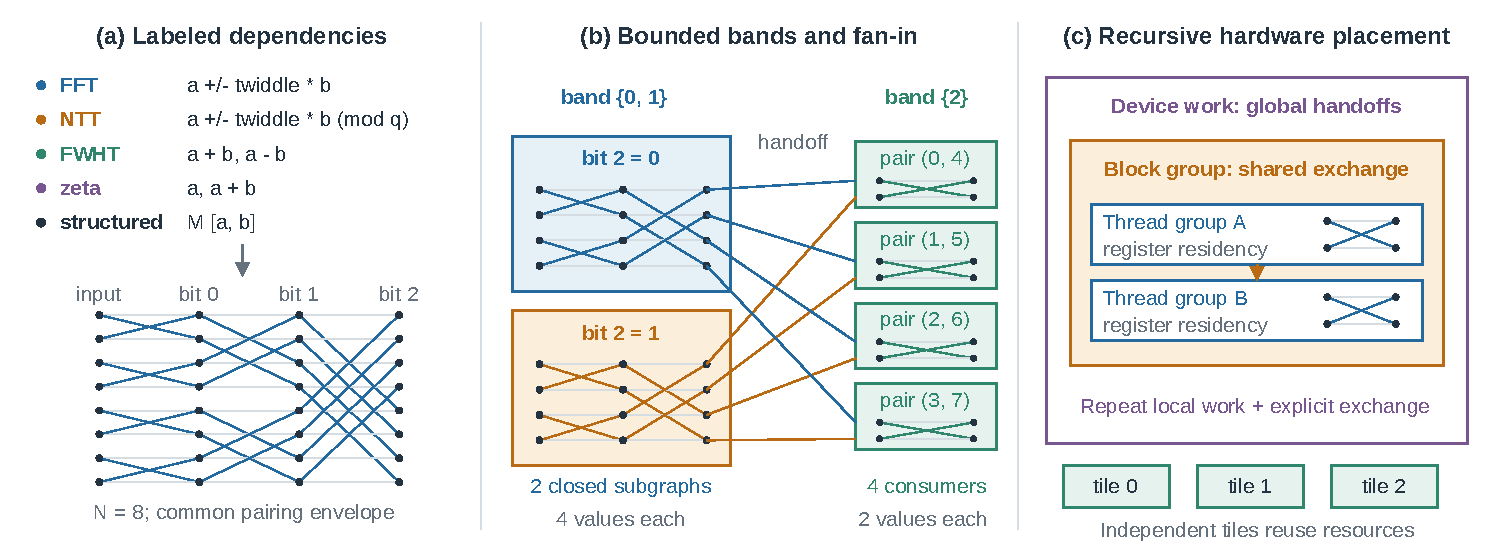
\includegraphics[width=\textwidth]{figures/drawio/exports/overview.pdf}
\caption{The organizing idea. (a) Butterfly families retain their arithmetic
labels on a common dependency construction. (b) Stage and data choices form
bounded subgraphs and explicit handoffs. (c) The construction repeats across
storage scopes, combining local residency with streamed execution. This is a
construction schematic, not a measured schedule.}
\label{fig:overview}
\end{figure*}

GPUs already provide strong arithmetic kernels and mature transform libraries
~\cite{cufft,vkfft,gpuntt,daofht}. However, a fast local core does not determine
the performance of a complete transform. Materializing every stage increases
traffic and launch overhead. Retaining more stages reduces these boundaries
but consumes registers and shared memory, potentially reducing occupancy.
A producer layout may further penalize the next consumer. These effects
couple computation, communication, and available parallel work across
transform lengths, batches, and hardware configurations. This makes the
problem more than selecting a faster pair operation. A library must decide
which dependencies to keep local and how to expose the remaining work without
turning each combination of operator, size, and device into a separate design.

Prior systems address important parts of this problem. SPIRAL and FFTX
unify transform descriptions and implementation generation
~\cite{spiral2005,fftx2018}. FlashFFTConv organizes FFT convolution around
tensor cores~\cite{flashfftconv2024}, and Welder propagates tile reuse
through computation graphs~\cite{welder2023}. These successes suggest that
the missing link is not an absence of tiling or search, but a reusable account
of which local regions and exchanges the butterfly dependencies permit.
Our question is more specific.
\textbf{Can butterfly dependencies define a reusable execution paradigm,
including both local work and the communication between local units?}
Section~\ref{sec:related} compares the organizing objects and scope of these
approaches.

We derive the execution unit from stage bits. Holding other index bits fixed
produces a \textbf{dependency-closed subgraph}, within which the selected
stages require no external values. Intersections between adjacent subgraphs
identify communication and readiness without expanding every scalar edge.
Arithmetic labels remain attached to the operations, allowing this construction
to serve FFT, NTT, FWHT, zeta, and structured stages without conflating their
semantics.

This construction supports \textbf{hierarchical hybrid dataflow}. At each
scope, stage and data positions can occupy spatial resources or reuse them
over time. A bounded subgraph retains intermediate values while independent
work streams through the resources. Repeating this choice across storage
scopes expresses workloads beyond any fixed local capacity. At a boundary,
\textbf{successor-aligned writeback} maps logical values to the consumer's
representation, potentially removing a separate reordering pass.

Our contributions are three linked pieces:
\begin{enumerate}
\item We define a \textbf{unified execution construction} from labeled
butterfly dependencies. Operator semantics, workload domains, and hardware
capabilities remain separate inputs to a joint mapping problem.
\item We define \textbf{hierarchical hybrid dataflow} through bounded
subgraph closure, residency, explicit communication, readiness, and
successor-aligned writeback. The construction scales by repeating the same
rules across storage scopes.
\item We realize and evaluate the construction with compatible cores, measured
services, bounded search, fixed-core controls, and profiler evidence. The
evaluation reports both gains and contracts where application integration is
still incomplete.
\end{enumerate}

\system{} realizes the method through block-level and resident subgraph
execution. It binds compatible cores, generates layouts and schedules, and
selects checked implementations under a finite budget. Our evaluation connects
library comparisons to fixed-core controls and trace diagnostics. The bounded
A100 80GB screen measures FFT geometric-mean latency ratios of 1.103$\times$
and 1.353$\times$ over cuFFT for its FP32 and FP64 requests, with separate
NTT and FWHT gains under their stated contracts. More directly,
changing organization improves both tested FFT cores by about 1.22$\times$.
These controls test whether the shared execution method contributes beyond
the arithmetic core itself. We first develop the organization problem from
the shared graph and prior approaches, then derive the method and its GPU
realization. The evaluation follows the same chain from overall efficiency
to the mechanisms and limits behind it.
